\documentclass[10pt, french]{article}
\usepackage[landscape, hmargin=1cm, vmargin=1.7cm]{geometry}
\usepackage{tikz,pgfplots}
\usepackage{csquotes}
\usepackage{tabularx}
\setlength{\extrarowheight}{7pt}

%% -----------------------------
%% Préambule
%% -----------------------------
% !TEX encoding = UTF-8 Unicode
% LaTeX Preamble for all cheatsheets
% Author : Gabriel Crépeault-Cauchon

% HOW-TO : copy-paste this file in the same directory as your .tex file, and add in your preamble the next command right after you have specified your documentclass : 
% \input{preamble-cheatsht.tex}
% ---------------------------------------------
% ---------------------------------------------

% Extra note : this preamble creates document that are meant to be used inside the multicols environment. See the documentation on internet for further information.

%% -----------------------------
%% Encoding packages
%% -----------------------------
\usepackage[utf8]{inputenc}
\usepackage[T1]{fontenc}
\usepackage{babel}
\usepackage{lmodern}
\usepackage[colorinlistoftodos]{todonotes}
%% -----------------------------
%% Variable definition
%% -----------------------------
\def\auteur{\href{https://github.com/ressources-act/Guide_de_survie_en_actuariat/blob/master/02_Cheatsheets/contributeurs/contributeurs-cheatshts.pdf}{\faGithub \ Liste des contributeurs}}
\def\BackgroundColor{white}
\usepackage{xargs} % for more logical new function creation

%% -----------------------------
%% Margin and layout
%% -----------------------------
% Determine the margin for cheatsheet
\usepackage[landscape, hmargin=1cm, vmargin=1.7cm]{geometry}
\usepackage{multicol}

% Remove automatic indentation after section/subsection title.
\setlength{\parindent}{0cm}

% Save space in cheatsheet by removing space between align environment and normal text.
\usepackage{etoolbox}
\newcommand{\zerodisplayskips}{%
  \setlength{\abovedisplayskip}{0pt}%
  \setlength{\belowdisplayskip}{0pt}%
  \setlength{\abovedisplayshortskip}{0pt}%
  \setlength{\belowdisplayshortskip}{0pt}}
\appto{\normalsize}{\zerodisplayskips}
\appto{\small}{\zerodisplayskips}
\appto{\footnotesize}{\zerodisplayskips}

%% -----------------------------
%% URL and links
%% -----------------------------
\usepackage{hyperref}
\hypersetup{colorlinks = true, urlcolor = gray!70!white, linkcolor = black}

%% -----------------------------
%% Document policy (uncomment only one)
%% -----------------------------
%	\usepackage{concrete}
	\usepackage{mathpazo}
%	\usepackage{frcursive} %% permet d'écrire en lettres attachées
%	\usepackage{aeguill}
%	\usepackage{mathptmx}
%	\usepackage{fourier} 

%% -----------------------------
%% Math configuration
%% -----------------------------
\usepackage[fleqn]{amsmath}
\usepackage{amsthm,amssymb,latexsym,amsfonts}
\usepackage{gensymb}
\usepackage{empheq}
\usepackage{numprint}
\usepackage{dsfont} % Pour avoir le symbole du domaine Z
%\usepackage{bigints} % pour des gros intégrales
% Mathematics shortcuts
\usepackage{scalerel,stackengine,amsmath}
\newcommand\equalhat{\mathrel{\stackon[1.5pt]{=}{\stretchto{%
    \scalerel*[\widthof{=}]{\wedge}{\rule{1ex}{3ex}}}{0.5ex}}}}
\newcommand{\reels}{\mathbb{R}}
\newcommand{\entiers}{\mathbb{Z}}
\newcommand{\naturels}{\mathbb{N}}
\newcommand{\eval}{\biggr \rvert}
\usepackage{cancel}
\newcommand{\derivee}[1]{\frac{\partial}{\partial #1}}
\newcommand{\prob}[1]{\Pr \left( #1 \right)}
\newcommand{\esp}[1]{\mathrm{E} \left[ #1 \right]} % espérance
\newcommand{\variance}[1]{\mathrm{Var} \left( #1   \right)}
\newcommand{\covar}[1]{\mathrm{Cov} \left( #1   \right)}
\newcommand{\laplace}{\mathcal{L}}
\newcommand{\deriv}[3][]{\frac{\partial^{#1}#3}{\partial #2^{#1}}}
\newcommand{\e}[1]{\mathrm{e}^{#1}}
\newcommand{\te}[1]{\text{exp}\left\{#1\right\}}
\DeclareMathSymbol{\shortminus}{\mathbin}{AMSa}{"39}
%%	Example usage:	\sumz{n}{i = 1} <=> \overset{n}{\underset{i = 1}{\sum}}
\newcommand{\sumz}[2]{\overset{#1}{\underset{#2}{\sum}}}
%%	Example usage:	\limz{h}{0} <=> \underset{h \rightarrow 0}{\lim}
\newcommand{\limz}[2]{\underset{#1 \rightarrow #2}{\lim}}
%%	Example usage:	\LVx{h}	<=>	\actsymb[h]{L}{}[]
%%					\LVx[n]{h}	<=>	\actsymb[h]{L}{}[n]
\newcommand{\LVx}[2][]{\actsymb[#2]{L}{}[#1]}
\DeclareMathOperator*{\argmax}{arg\,max}
\DeclareMathOperator*{\argmin}{arg\,min}
%%%	\icbox{<frame color>}{<background color>}{<text>}
\newcommandx{\icbox}[3][1 = bleudefrance, 2 = beaublue]{\fcolorbox{#1}{#2}{#3}}
%%	other good color combo is azure(colorwheel) arsenic
\usepackage{longfbox}
%	voir cette page, paquetage avec CSS https://ctan.math.illinois.edu/macros/latex/contrib/longfbox/longfbox.html
\newfboxstyle{rappel}{
	background-color = tealblue!20!white, 
	border-style = outset,
	breakable = true,
%	
	border-color = tealblue,
	border-radius = 1ex, 
%
	padding-bottom = 0.2ex,
	padding-top = 0.2ex,
	padding-left = 0.4ex,
	padding-right = 0.4ex,
%	
	border-top-width = 0.3ex,
	border-bottom-width = 0.3ex,
%
	border-left-width = 1ex, 
	border-bottom-left-radius = 0.2ex,
%	
	border-right-width = 1ex, 
	border-top-right-radius = 0.2ex,
%	
}
\newfboxstyle{formula}{ 
	background-color = beaublue, 
	border-color = bleudefrance
}
\newfboxstyle{imphl}{ 
	padding = 0pt,
	margin = 0pt,
	baseline-skip = false,
	background-color = palechestnut!60!white, 
	border-color = white
}
\newfboxstyle{conditions}{ 
	background-color = palechestnut, 
	border-color = red
}
\newcommandx{\rcbox}[3][1 = bleudefrance, 2 = beaublue]{\lfbox[border-radius = 0.5ex, background-color = #2, border-color = #1]{#3}}

% To indicate equation number on a specific line in align environment
\newcommand\numberthis{\addtocounter{equation}{1}\tag{\theequation}}

%
% Actuarial notation packages
%
\usepackage{actuarialsymbol}
\usepackage{actuarialangle}

%
% Matrix notation for math symbols (\bm{•})
%
\usepackage{bm}
% Matrix notation variable (bold style)
\newcommand{\matr}[1]{\mathbf{#1}}



%% -----------------------------
%% tcolorbox configuration
%% -----------------------------
\usepackage[most]{tcolorbox}
\tcbuselibrary{xparse}
\tcbuselibrary{breakable}

%%
%% Coloured box "definition" for definitions
%%
\DeclareTColorBox{definition}{ o }				% #1 parameter
{
	colframe=black,colback=white, % color of the box
	breakable, 
	pad at break* = 0mm, 						% to split the box
	title = {#1},
	after title = {\large \hfill \faBook},
}
%%
%% Coloured box "definition2" for definitions
%%
\DeclareTColorBox{definitionNOHFILL}{ o }				% #1 parameter
{
	colframe=blue!60!green,colback=blue!5!white, % color of the box
	pad at break* = 0mm, 						% to split the box
	title = {#1},
	before title = {\faBook \quad },
	breakable
}
%%
%% Coloured box "definition2" for definitions
%%
\DeclareTColorBox{definitionNOHFILLsub}{ o }				% #1 parameter
{
	colframe=blue!40!green,colback=blue!5!white, % color of the box
	pad at break* = 0mm, 						% to split the box
	title = {#1},
	before title = {\faNavicon \quad }, %faBars  faGetPocket
	breakable
}
%%
%% Coloured box "definition3" for propriétés
%%
\DeclareTColorBox{definitionNOHFILLprop}{ o }				% #1 parameter
{
	colframe=amber(sae/ece),colback=amber(sae/ece)!5!white, % color of the box
	pad at break* = 0mm, 						% to split the box
	title = {#1},
	before title = {\faGetPocket \quad }, %faBars  faGetPocket
	breakable
}
%%
%% Coloured box "definition3" for propriétés
%%
\DeclareTColorBox{definitionNOHFILLpropos}{ o }				% #1 parameter
{
	colframe=carmine,colback=carmine!5!white, % color of the box
	pad at break* = 0mm, 						% to split the box
	title = {#1},
	before title = {\faColumns \quad }, %\faEllipsisH  faColumns
	breakable
}


%%
%% Coloured box "algo" for algorithms
%%
\newtcolorbox{algo}[ 1 ]
{
	colback = blue!5!white,
	colframe = blue!75!black,
	title=#1,
	fonttitle = \bfseries,
	breakable
}
%%
%% Coloured box "conceptgen" for points adding to a concept's deifintion
%%
\newtcolorbox{conceptgen}[ 1 ]
{
	breakable,
	colback = beaublue,
	colframe = airforceblue,
	title=#1,
	fonttitle = \bfseries
}
%%
%% Coloured box "rappel" pour rappel de formules
%%
\DeclareTColorBox{conceptgen_enhanced}{ o }
{
	enhanced,
	title = #1,
	colback=beaublue, % color of the box
%	colframe=blue(pigment),
%	colframe=arsenic,	
	colbacktitle=airforceblue,
	fonttitle = \bfseries,
	breakable,
	boxed title style={size=small,colframe=arsenic} ,
	attach boxed title to top center = {yshift=-3mm,yshifttext=-1mm},
}
%%
%% Coloured box "probch1" pour formules relatives au 1er chapitre de prob
%%
\newtcolorbox{probch1}[ 1 ]
{
	colback = ao(english)!40!white,
	colframe = forestgreen(traditional),
	fonttitle = \bfseries,	
	breakable,
	title=#1
}
%%
%% Coloured box "probch2" pour formules relatives au 2e chapitre de prob
%%
\newtcolorbox{probch2}[ 1 ]
{
	colback = orange!50!white,
	colframe = burntorange,
	fonttitle = \bfseries,	
	breakable,
	title=#1
}
%%
%% Coloured box "axioms" pour formules relatives à la dernière partie du chapitre 2 de prob
%%
\newtcolorbox{axioms}[ 1 ]
{
	colback = blue!10!white,
	colframe = blue!70!white,
	fonttitle = \bfseries,	
	breakable,
	title=#1
}
%%
%% Coloured box "probch3" pour formules relatives au 3ème chapitre de prob
%%
\newtcolorbox{probch3}[ 1 ]
{
	colback = ruddypink,
	colframe = burgundy,
	fonttitle = \bfseries,	
	breakable,
	title=#1
}
%%
%% Coloured box "formula" for formulas
%%
\newtcolorbox{formula}[ 1 ]
{
	colback = green!5!white,
	colframe = green!70!black,
	breakable,
	fonttitle = \bfseries,
	title=#1
}
%%
%% Coloured box "formula" for formulas
%%
\DeclareTColorBox{algo2}{ o }
{
	enhanced,
	title = #1,
	colback=blue!5!white,	
	colbacktitle=blue!75!black,
	fonttitle = \bfseries,
	breakable,
	boxed title style={size=small,colframe=arsenic} ,
	attach boxed title to top center = {yshift=-3mm,yshifttext=-1mm},
}
%%
%% Coloured box "examplebox" for formulas
%%
\newtcolorbox{examplebox}[ 1 ]
{
	colback = beaublue,
	colframe = amethyst,
	breakable,
	fonttitle = \bfseries,title=#1
}
%%
%% Coloured box "rappel" pour rappel de formules
%%
\newtcolorbox{rappel}[ 1 ]
{
	colback = ashgrey,
	colframe = arsenic,
	breakable,
	fonttitle = \bfseries,title=#1
}
%%
%% Coloured box "rappel" pour rappel de formules
%%
\DeclareTColorBox{rappel_enhanced}{ o }
{
	enhanced,
	title = #1,
	colback=ashgrey, % color of the box
%	colframe=blue(pigment),
%	colframe=arsenic,	
	colbacktitle=arsenic,
	fonttitle = \bfseries,
	breakable,
	boxed title style={size=small,colframe=arsenic} ,
	attach boxed title to top center = {yshift=-3mm,yshifttext=-1mm},
}
%%
%% Coloured box "notation" for notation and terminology
%%
\DeclareTColorBox{distributions}{ o }			% #1 parameter
{
	enhanced,
	title = #1,
	colback=gray(x11gray), % color of the box
%	colframe=blue(pigment),
	colframe=arsenic,	
	colbacktitle=aurometalsaurus,
	fonttitle = \bfseries,
	boxed title style={size=small,colframe=arsenic} ,
	attach boxed title to top center = {yshift=-3mm,yshifttext=-1mm},
	breakable
%	left=0pt,
%  	right=0pt,
%    box align=center,
%    ams align*
%  	top=-10pt
}
\newtcolorbox{contrib}[ 1 ]
{
	colback = babyblueeyes,
	colframe = airforceblue,
	fonttitle = \bfseries,
	title = {#1},
	valign = center
}

%% -----------------------------
%% Graphics and pictures
%% -----------------------------
\usepackage{graphicx}
\usepackage{pict2e}
\usepackage{tikz}

%% -----------------------------
%% insert pdf pages into document
%% -----------------------------
\usepackage{pdfpages}

%% -----------------------------
%% Color configuration
%% -----------------------------
\usepackage{color, soulutf8, colortbl}


%
%	Colour definitions
%
\definecolor{armygreen}{rgb}{0.29, 0.33, 0.13}	%	army
\definecolor{asparagus}{rgb}{0.53, 0.66, 0.42}	% pastel green militariesque
\definecolor{britishracinggreen}{rgb}{0.0, 0.26, 0.15}
\definecolor{calpolypomonagreen}{rgb}{0.12, 0.3, 0.17}
\definecolor{darkgreen}{rgb}{0.0, 0.2, 0.13}
\definecolor{lightgreen}{rgb}{0.2, 0.95, 0.2}

\definecolor{antiquebrass}{rgb}{0.8, 0.58, 0.46}	% brown-ish light cardboard color

\definecolor{blue(munsell)}{rgb}{0.0, 0.5, 0.69}
\definecolor{blue(matcha)}{rgb}{0.596, 0.819, 1.00}
\definecolor{blue(munsell)-light}{rgb}{0.5, 0.8, 0.9}
\definecolor{bleudefrance}{rgb}{0.19, 0.55, 0.91}
\definecolor{blizzardblue}{rgb}{0.67, 0.9, 0.93}	%	mr.freeze light baby blue 
\definecolor{bondiblue}{rgb}{0.0, 0.58, 0.71}	%	darker cyan type inidgo blue
\definecolor{blue(pigment)}{rgb}{0.2, 0.2, 0.6}
\definecolor{bluebell}{rgb}{0.64, 0.64, 0.82}
\definecolor{airforceblue}{rgb}{0.36, 0.54, 0.66}
\definecolor{beaublue}{rgb}{0.74, 0.83, 0.9}    % almost white
\definecolor{blue_rectangle}{RGB}{83, 84, 244}		% ACT-2004
\definecolor{cobalt}{rgb}{0.0, 0.28, 0.67}	% nice light blue-ish
\definecolor{ballblue}{rgb}{0.13, 0.67, 0.8}	%	almost green ish blue ish
\definecolor{babyblueeyes}{rgb}{0.63, 0.79, 0.95}

\definecolor{indigo(web)}{rgb}{0.29, 0.0, 0.51}	% purple-ish
\definecolor{antiquefuchsia}{rgb}{0.57, 0.36, 0.51}	%	pastel matte (darkerish) purple ish
\definecolor{darkpastelpurple}{rgb}{0.59, 0.44, 0.84}	%	pretty purple
\definecolor{gray(x11gray)}{rgb}{0.75, 0.75, 0.75}
\definecolor{aurometalsaurus}{rgb}{0.43, 0.5, 0.5}
\definecolor{bulgarianrose}{rgb}{0.28, 0.02, 0.03}	%	dark maroon type 
\definecolor{pastelred}{rgb}{1.0, 0.41, 0.38}		%	light red pinktinybit ish
\definecolor{lightmauve}{rgb}{0.86, 0.82, 1.0}
\definecolor{eggshell}{rgb}{0.94, 0.92, 0.84}
\definecolor{azure(colorwheel)}{rgb}{0.0, 0.5, 1.0}
\definecolor{darkgreen}{rgb}{0.0, 0.2, 0.13}			
\definecolor{ao(english)}{rgb}{0.0, 0.5, 0.0}		% prertty apple dark pastel (light) green
\definecolor{green_rectangle}{RGB}{131, 176, 84}		% ACT-2004
\definecolor{red_rectangle}{RGB}{241,112,113}		% ACT-2004
\definecolor{amethyst}{rgb}{0.6, 0.4, 0.8}
\definecolor{amethyst-light}{rgb}{0.6, 0.4, 0.8}
\definecolor{ruddypink}{rgb}{0.88, 0.56, 0.59}

\definecolor{amber(sae/ece)}{rgb}{1.0, 0.49, 0.0} 	%	pretty orange ish
\definecolor{burntsienna}{rgb}{0.91, 0.45, 0.32}		%%	lighter pastel orange
\definecolor{burntorange}{rgb}{0.8, 0.33, 0.0}		%%	similar but deeper orange
\definecolor{orange-red}{rgb}{1.0, 0.27, 0.0}

\definecolor{tealblue}{rgb}{0.21, 0.46, 0.53}

\definecolor{battleshipgrey}{rgb}{0.52, 0.52, 0.51}  % lilght ish gray
\definecolor{ashgrey}{rgb}{0.7, 0.75, 0.71}			% dark grey-black-ish
\definecolor{arsenic}{rgb}{0.23, 0.27, 0.29}			% light green-beige-ish gray
\definecolor{gray(x11gray)}{rgb}{0.75, 0.75, 0.75}

\definecolor{carmine}{rgb}{0.59, 0.0, 0.09} 			% deep red
\definecolor{amaranth}{rgb}{0.9, 0.17, 0.31}
\definecolor{brickred}{rgb}{0.8, 0.25, 0.33}
\definecolor{chestnut}{rgb}{0.8, 0.36, 0.36}		% pink red ish light
\definecolor{palechestnut}{rgb}{0.87, 0.68, 0.69}
\definecolor{pastelred}{rgb}{1.0, 0.41, 0.38}
\definecolor{forestgreen(traditional)}{rgb}{0.0, 0.27, 0.13}
%
% Useful shortcuts for coloured text
%
\newcommand{\orange}{\textcolor{orange}}
\newcommand{\red}{\textcolor{red}}
\newcommand{\cyan}{\textcolor{cyan}}
\newcommand{\blue}{\textcolor{blue}}
\newcommand{\green}{\textcolor{green}}
\newcommand{\purple}{\textcolor{magenta}}
\newcommand{\yellow}{\textcolor{yellow}}

%% -----------------------------
%% Enumerate environment configuration
%% -----------------------------
%
% Custum enumerate & itemize Package
%
\usepackage{enumitem}
%
% French Setup for itemize function
%
\frenchbsetup{StandardItemLabels=true}
%
% Change default label for itemize
%
\renewcommand{\labelitemi}{\faAngleRight}


%% -----------------------------
%% Tabular column type configuration
%% -----------------------------
\newcolumntype{C}{>{$}c<{$}} % math-mode version of "l" column type
\newcolumntype{L}{>{$}l<{$}} % math-mode version of "l" column type
\newcolumntype{R}{>{$}r<{$}} % math-mode version of "l" column type
\newcolumntype{f}{>{\columncolor{green!20!white}}p{1cm}}
\newcolumntype{g}{>{\columncolor{green!40!white}}m{1.2cm}}
\newcolumntype{a}{>{\columncolor{red!20!white}$}p{2cm}<{$}}	% ACT-2005
% configuration to force a line break within a single cell
\usepackage{makecell}


%% -----------------------------
%% Fontawesome for special symbols
%% -----------------------------
\usepackage{fontawesome}

%% -----------------------------
%% Section Font customization
%% -----------------------------
\usepackage{sectsty}
\sectionfont{\color{\SectionColor}}
\subsectionfont{\color{\SubSectionColor}}
\subsubsectionfont{\color{\SubSubSectionColor}}

%% -----------------------------
%% Footer/Header Customization
%% -----------------------------
\usepackage{lastpage}
\usepackage{fancyhdr}
\pagestyle{fancy}

%
% Header
%
\fancyhead{} 	% Reset
\fancyhead[L]{Aide-mémoire pour~ \cours ~(\textbf{\sigle})}
\fancyhead[R]{\auteur}

%
% Footer
%
\fancyfoot{}		% Reset
\fancyfoot[R]{\thepage ~de~ \pageref{LastPage}}
\fancyfoot[L]{\href{https://github.com/ressources-act/Guide_de_survie_en_actuariat}{\faGithub \ ressources-act/Guide de survie en actuariat}}
%
% Page background color
%
\pagecolor{\BackgroundColor}




%% END OF PREAMBLE
% ---------------------------------------------
% ---------------------------------------------
%% -----------------------------
%% Variable definition
%% -----------------------------
%% -----------------------------
%% Footer and header customization
%% -----------------------------
\def\cours{Analyse probabiliste des risques actuariels}
\def\sigle{ACT-1002}
\fancyfoot[R]{\thepage ~de~ \pageref{LastPage}}
\setlist{leftmargin=*}

%% -----------------------------
%% Colour setup for sections
%% -----------------------------
\def\SectionColor{cobalt}
\def\SubSectionColor{azure(colorwheel)}
\def\SubSubSectionColor{azure(colorwheel)}
\definecolor{burgundy}{rgb}{0.5, 0.0, 0.13}

%% -----------------------------
%% Definition of LaTex math commands
%% -----------------------------
\newcommand{\norm}[1]{\left\lVert#1\right\rVert}

%% -----------------------------
%% Setup for Venn diagrams
%% -----------------------------
\def\firstrectangle{(0,0) rectangle (7, 4)}
\def\firstcircle{(2.5,2) circle (1.5cm)}
\def\secondcircle{(4.5, 2) circle (1.5cm)}
\colorlet{circle edge}{blue!50}
\colorlet{circle area}{blue!20}\tikzset{filled/.style={fill=circle area, draw=circle edge, thick},
    outline/.style={draw=circle edge, thick}}

%% -----------------------------
%% Setup for appendice tables
%% -----------------------------
\newcolumntype{Y}{>{\centering\arraybackslash}X}

%% French quotation marks
\MakeOuterQuote{"}


\begin{document}
\begin{center}
	\textsc{\Large Contributeurs}\\[0.5cm] 
\end{center}
\input{contributeurs/contrib-ACT1002}

\newpage

\begin{multicols*}{2}

\section{Analyse combinatoire}
\subsection{Outils d'analyse combinatoire}
\begin{definitionNOHFILL}[Principe de base de comptage]
Pour une expérience 1 avec $m$ résultats possibles et une expérience 2 avec $n$ résultats possibles, il y a $m * n$ résultats possibles pour les deux expériences ensemble. Ce résultat peut être généralisé pour r expériences, où il y aurait $n_1*n_2*...{}*n_r$ possibilités.
\end{definitionNOHFILL}

\begin{definitionNOHFILL}[Permutations]
Lorsqu'on s'intéresse au nombre d'arrangements possibles de $n$ éléments \textbf{distincts} (\textbf{donc qu'on s'intéresse à l'ordre de ces éléments}), le nombre total de possibilités est représenté par $n!$.\\
\\
Lorsqu'on s'intéresse au nombre d'arrangements possibles de $n$ éléments de $k$ types différents dont $n_1$ sont identiques, $n_2$ sont identiques, ..., $n_k$ sont identiques (\textbf{donc qu'on s'intéresse à l'ordre de ces éléments}), le nombre total de possibilités est représenté par : $$\frac{n!}{n_1!*n_2!* ... *n_k!}.$$
\end{definitionNOHFILL}

\begin{definitionNOHFILL}[Combinaisons]
Lorsqu'on s'intéresse au nombre de groupe possibles de $k$ éléments parmi $n$ (\textbf{donc qu'on ne s'intéresse pas à l'ordre de ces éléments}), le nombre total de possibilités est représenté par $\binom{n}{k}$.
\end{definitionNOHFILL}

\begin{distributions}[Notation]
Dans l'exemple précédent, on peut observer la notation propre au coefficient binomial. Ce dernier peut être réécrit de la façon suivante : $$\binom{n}{k} = \frac{n!}{k!(n-k)!}.$$
\end{distributions}

\begin{definitionNOHFILLprop}[Relation de Pascal]
$$\binom{n}{k} = \binom{n-1}{k-1}+\binom{n-1}{k}$$ 
\end{definitionNOHFILLprop}

\begin{formula}{Exemples classiques sur les permutations et les combinaisons}

\begin{enumerate}[label = \rectangled{\arabic*}{teal}]
	\item \textbf{Combien de façons différentes peut-on placer $4$ livres distincts sur une étagère?}
	C'est une permutation entre 4 éléments. La réponse est $4!$.\\
	\item \textbf{Combien d'arrangements ordonnés différents peut-on faire avec les lettres du mot LAVAL?}\\
	\\
	 C'est une permutation d'un ensemble qui contient deux paires d'éléments semblables. Donc, la réponse est $\frac{5!}{2!2!1!}$.
	 \\
	\item \textbf{Combien de façons différentes peut-on distribuer 12 cadeaux différents à 4 personnes?} \\
	\\
	Attention! Ici, il faut bien voir que, pour chaque cadeau, il y a 4 possibilités (et  \textbf{non} qu'il y a 12 possibilités pour chaque personne!). Donc, la réponse est $4^{12}$. \\
\\
Dans ce numéro, il faut aussi faire attention au fait qu'on précise que les cadeaux sont distincts (donc qu'on différencie les cadeaux). Si ce n'était pas le cas, il s'agirait d'un numéro sur des éléments indissociables.\\
	\item \textbf{Combien de groupes différents de 2 jouets peut-on faire avec 6 jouets ?}\\
	La réponse est $\binom{6}{2}$.
\end{enumerate}
\end{formula}

\begin{definitionNOHFILL}[Coefficient multinomial]
La généralisation du coefficient binomial va comme suit:\\ $$\binom{n}{k_1, k_2, ..., k_m} = \frac{n!}{k_1!* k_2!*  ... *k_m!}$$\\ où $n = \sum_{i = 1}^{m} k_i$. Cette formule est utile si on veut séparer des éléments entre plusieurs groupes.
\end{definitionNOHFILL}
\begin{definitionNOHFILL}[Coefficient multinomial (suite)]
Par exemple, si on a 10 jouets à séparer entre 3 enfants, et que le premier en veut 5, le deuxième en veut 2, et le troisième en veut 3, le nombre de possibilités est donné par $\binom{10}{5, 2, 3}.$ \\

Si, cette fois-ci, on différencie les groupes, et qu'on ne sait pas quel groupe aura quel nombre d'objets, il faut multiplier le coefficient multinomial de la façon suivante: 
$$ coefficient\ multinomial * \frac{n!}{n_1!*n_2!* ... *n_n!}$$\\ où $n$ correspond au nombre total de groupes et $n_i$ correspond au nombre de groupes dans lesquels $i$ éléments ont été placés. \\
\\
Par exemple, si cette fois-ci on dit qu'il faut séparer 10 jouets à travers 3 enfants en donnant 3 jouets à 2 enfants et 4 jouets à l'autre enfant, sans spécifier quel enfant recevra 4 jouets, le résultat sera :\\ $$ \binom{10}{3, 3, 4} * \frac{3!}{1!2!}.$$
\end{definitionNOHFILL}

\begin{definitionNOHFILLprop}[Théorème binomial]
$$(x + y)^ n = \sum_{k=0}^{n} \binom{n}{k} x^k y^{n-k}$$
\end{definitionNOHFILLprop}

\begin{definitionNOHFILLprop}[Théorème multinomial]
$$(x_1 + x_2 + ... + x_r)^n = \sum_{n_1 + n_2 + ... + n_r = n} \binom{n}{n_1, n_2, ..., n_r}x_1^{n_1} x_2^{n_2} ... x_r^{n_r}$$ 
\end{definitionNOHFILLprop}

\subsection{Nombre de solutions entières}
\begin{definitionNOHFILLsub}[Nombre de solutions entières] Dans certains cas, on s'intéressera au nombre de façons qu'on peut distribuer des éléments \textbf{indissociables} dans des contenants. Ainsi, c'est le nombre d'éléments dans chaque contenant qui nous intéressent, et non quel élément va dans quel contenant. 
\end{definitionNOHFILLsub}
\begin{definitionNOHFILLsub}[Nombre de solutions entières (suite)]
On peut ramener ce problème à une équation de la forme suivante :\\ $$k_1+k_2+ ... +k_r = n$$\\ où $k_i$ correspond au nombre d'éléments dans le contenant $i$ et $n$ le nombre d'éléments à placer dans les contenants. On essaie donc de trouver le nombre de combinaisons possibles de $k_1$, $k_2$, ..., $k_r$. Voici une façon de résoudre les problèmes reliés aux nombres de solutions entières:

\begin{itemize}
\item S'il faut placer au moins un élément dans chaque contenant (donc $k_i \geq 1$ pour tout $i$), on peut appliquer la formule : $\binom{n-1}{k-1}$. 
\item S'il n'y a pas de contraintes en lien avec le nombre d'éléments à placer (donc $k_i \geq 0$ pour tout $i$), on peut appliquer la formule : $\binom{n+k-1}{k-1}$.
\item Si on mentionne dans l'énoncé qu'on peut ne pas distribuer tous les éléments, on rajoute un contenant de plus à l'équation, qui comprend tous les éléments non distribués (le nombre d'éléments dans ce contenant sera plus grand ou égal à 0).
\item S'il y a une contrainte supérieure, on fait le problème sans tenir compte de cette contrainte, et on enlève le nombre de cas ne respectant pas la contrainte une fois le problème fait.
\item Si la contrainte inférieure varie d'un contenant à un autre, ou si elle est supérieure à 2, on applique la stratégie suivante.
\end{itemize}

Exemple : il y a 10 balles à placer dans trois urnes. La première urne n'a aucune contrainte, la deuxième urne doit contenir au minimum 1 balle et la troisième urne doit contenir au minimum 3 balles. On obtient l'équation ci-dessous : \\
$$k_1+k_2+k_3 = 10.$$ \\
Ici, on va poser $y_1 = k_1 + 1$, $y_2 = k_2$ et $y_3 = k_3 - 2$ afin que $y_i \geq 1$ pour tout $i$. On réécrit l'équation ci-dessus de la façon suivante: \\ $$y_1 - 1 + y_2+ y_3 + 2 = 10$$ 
$$y_1 + y_2+ y_3 = 9.$$\\ On peut par la suite calculer le nombre de possibilités en utilisant la formule lorsque le nombre d'éléments dans chaque contenant doit être plus grand ou égal à 1 : $\binom{9-1}{3-1} = \binom{8}{2}$ possibilités.

\end{definitionNOHFILLsub}


\pagebreak
\section{Axiomes de probabilité}
\subsection{Définitions importantes}
\begin{definitionNOHFILL}[Expérience aléatoire]
Une expérience aléatoire est un processus où on ne peut pas prédire avec certitude le résultat. 
\end{definitionNOHFILL}
\begin{definitionNOHFILL}[Espace échantillonnal]
L'espace échantillonnal est l'ensemble des résultats possibles d'une expérience aléatoire. On dénote cet espace par $\Omega$ ou $S$.
\end{definitionNOHFILL}
\begin{definitionNOHFILL}[Événement]
Un événement est un sous-ensemble d'un espace échantillonnal. On dénote l'événement par une lettre majuscule $A$, $B$, $C$, etc.
\end{definitionNOHFILL}
\subsection{Opérations sur les ensembles}
\begin{description} 
\item [L'union ({$\cup$}) :] On peut le voir comme un "ou". Lorsqu'il est utilisé, on s'intéresse à savoir si un résultat est présent dans au moins un des ensembles impliqués. 
\end{description}
\begin{itemize}
  	\item	Si l'événement $A$ est d'avoir 3 sur un dé et l'événement $B$ est d'avoir 4 sur ce même dé, les résultats possibles de $ A \cup B$ sont 3 et 4.
\end{itemize}
\begin{center}
 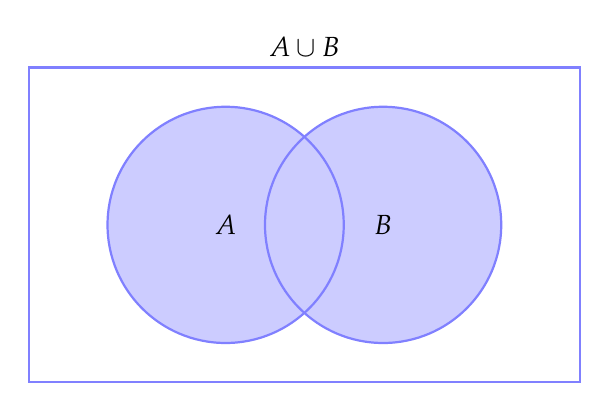
\begin{tikzpicture}
    \draw[outline] \firstrectangle;
    \draw[filled] \firstcircle node {$A$}
                  \secondcircle node {$B$};
    \node[anchor=south] at (current bounding box.north) {$A \cup B$};
\end{tikzpicture}
\end{center}
\columnbreak
\begin{description} 
 \item[L'intersection ({$\cap$}) :] On peut le voir comme un "et". Lorsqu'il est utilisé, on s'intéresse à savoir si un résultat est présent dans tous les ensembles impliqués.
\end{description}
\begin{itemize}
  	\item	Si l'événement $A$ est d'avoir un chiffre pair sur un dé et que l'événement $B$ est d'avoir 5 ou 6 sur ce même lancer de dé, le seul résultat possible de $A \cap B$ est 6, car 6 est un nombre pair et fait partie de l'ensemble $B$. 
  	\item Une notation alternative est de simplement écrire $AB$.
\end{itemize}
\begin{center}
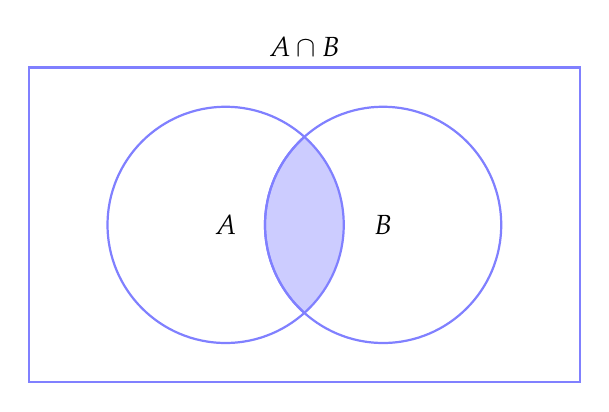
\begin{tikzpicture}
    \begin{scope}
        \clip \firstcircle;
        \fill[filled] \secondcircle;
    \end{scope}
    \draw[outline] \firstrectangle;
    \draw[outline] \firstcircle node {$A$};
    \draw[outline] \secondcircle node {$B$};
    \node[anchor=south] at (current bounding box.north) {$A \cap B$};
\end{tikzpicture}
\end{center}
\begin{description} 
 \item[Complémentaire :] Un événement $A^{c}$ est le complémentaire d'un événement A lorsqu'il correspond à tous les résultats de $\Omega$ excluant les résultats de $A$. 
\end{description}
\begin{itemize}
  	\item	Un exemple est l'événement "Avoir un nombre pair sur un dé"; un événement complémentaire serait donc "Avoir un nombre impair sur un dé".
  	\item   Le complémentaire d'un événement A est désigné par {$\overline{A}$}, $A^{c}$ et $A^{'}$.
\end{itemize}
\begin{center}
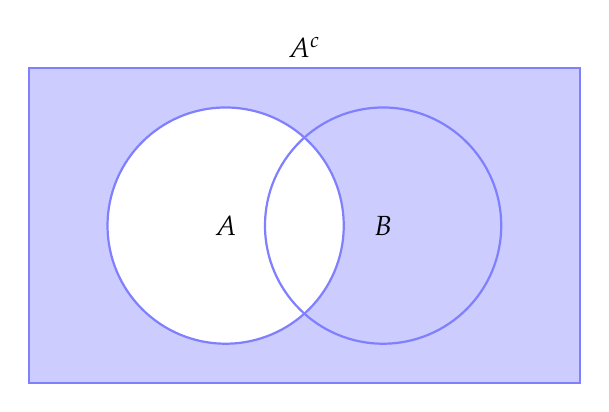
\begin{tikzpicture}
    \begin{scope}
    \fill [filled] \firstrectangle;
    \fill [white] \firstcircle;
    \end{scope}

    \draw[outline] \firstrectangle;
    \draw[outline] \firstcircle node {$A$};
    \draw[outline] \secondcircle node {$B$};
    \node[anchor=south] at (current bounding box.north) {$A^c$};
\end{tikzpicture}
\end{center}
\pagebreak
\begin{description} 
 \item[Inclusion ($\subset$) :] Afin de dire que l'événement B est compris dans l'événement A, on peut écrire le tout avec la notation suivante : $B \subset A$. On peut donc dire que tous les résultats de l'événement $B$ se retrouvent aussi dans l'événement $A$.
\end{description}
\begin{center}
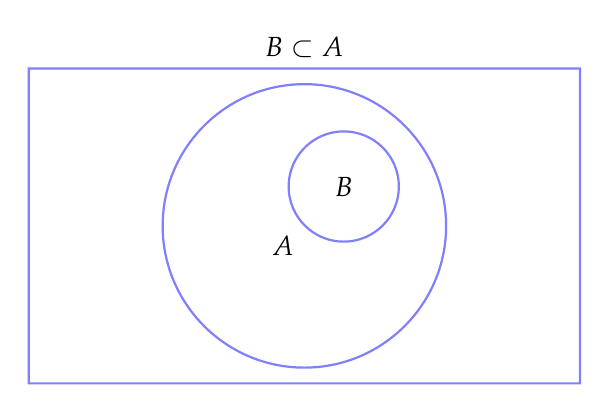
\begin{tikzpicture}
\draw[outline] \firstrectangle 
(3.5, 2) circle (1.8) node [text = black, below left]{$A$}
(4, 2.5) circle (0.7) node {$B$};
    \node[anchor=south] at (current bounding box.north) {$B \subset A$};
\end{tikzpicture}
\end{center}

\begin{definitionNOHFILL}[Événements mutuellement exclusifs]
Deux événements $A$ et $B$ sont dits mutuellement exclusifs lorsque l'intersection entre les deux événements est vide ($A \cap B = \emptyset$). C'est donc dire que $\Pr(A \cap B) = 0$. Autrement dit, les évènements n'ont aucun résultat en commun.
\end{definitionNOHFILL}

\begin{definitionNOHFILLprop}[Propriétés des ensembles]
\begin{description}
  \item[Commutativité :] 
  $$A_1	\cup	A_2	=	A_2 \cup A_1$$ $$A_1	\cap	A_2	=	A_2 \cap A_1$$
  \item[Associativité :] $$(A_1 \cup A_2)	\cup A_3	=	A_1 \cup		(A_2 \cup A_3)$$ $$(A_1 \cap A_2)	\cap A_3	=	A_1 \cap		(A_2 \cap A_3)$$
  \item[Distributivité :] $$(A_1 \cup A_2)	\cap A_3 = (A_1 \cap A_3) \cup (A_2 \cap A_3)$$ $$(A_1 \cap A_2)	\cup A_3 = (A_1 \cup A_3) \cap (A_2 \cup A_3)$$
  \item[Loi de DeMorgan :] $$(\bigcup_{i = 1}^{n} A_{i})^{c} = (\bigcap_{i=1}^{n} A_i^{c})$$ $$(\bigcap_{i = 1}^{n} A_{i})^{c} = (\bigcup_{i=1}^{n} A_i^{c})$$
\end{description}
\end{definitionNOHFILLprop}
\vfill\null
\columnbreak

\subsection{Axiomes de probabilité}
\begin{definitionNOHFILLprop}[Axiomes de probabilité]
Supposons que, pour chaque événement $A_i$ de $\Omega$ (espace échantillonnal d'une expérience aléatoire), il existe un nombre $\Pr(A_i)$. On peut appeler ce nombre la probabilité de $A_i$ si celle-ci satisfait les axiomes ci-dessous. Autrement dit, ces axiomes sont des règles que les probabilités se doivent de respecter: 

\begin{description}
  \item[1)] $0 \leq \Pr(A_i) \leq 1$
  \item[2)] $\Pr(\Omega)=1$
  \item[3)] Si $A_i$ $\cap$ $A_j$ = $\emptyset$ pour $i \neq j$ (\textbf{mutuellement exclusifs}), alors $$\Pr(\bigcup_{i = 1}^{n} A_i) = \sum_{i = 1}^{n} \Pr(A_i)$$
\end{description}
\end{definitionNOHFILLprop}

\begin{definitionNOHFILLprop}[Relations à savoir]

\begin{description}
  \item[1)] $\Pr(\emptyset) = 0$
  \item[2)] $\Pr(E^c) = 1 - \Pr(E)$
  \item[3)] Si $E \subset F$, alors $\Pr(E) \leq \Pr(F)$
  \item[4) (Formule de Poincaré)] \begin{align*} \Pr(E_1 \cup E_2 \cup ... \cup E_n) =& \sum_{i=1}^n \Pr(E_i) - \sum_{i_1<i_2} \Pr(E_{i_1} E_{i_2}) + ...+\\& (-1)^{r+1} \sum_{i_1<i_2<...<i_r} \Pr(E_{i_1}E_{i_2}...E_{i_r}) + ...+\\& (-1)^{n+1} \Pr(E_1E_2...E_n)
  \end{align*}
  \begin{itemize}
  \item À deux événements, on obtient :\\ $$\Pr(A \cup B) = \Pr(A) + \Pr(B) - \Pr(A \cap B)$$
  \item À trois événements, on obtient :\\
	\begin{align*}  
  \Pr(A \cup B \cup C) =& \Pr(A) + \Pr(B) + \Pr(C) - \\& \Pr(A \cap B) - \Pr(A \cap C) - \Pr(B \cap C) + \\& \Pr(	A \cap B \cap C)
  \end{align*}
  \end{itemize}
\end{description}
D'autres relations peuvent être déduites à l'aide d'un diagramme de Venn. Il faut toutefois utiliser la notation probabiliste à travers les calculs. Un diagramme de Venn avec de simples calculs \textbf{ne suffit pas} en examen.
\end{definitionNOHFILLprop}

\subsection{Résultats équiprobables}

\begin{definitionNOHFILL}[Résultats équiprobables]
Si chaque résultat de $\Omega$ a la même chance de se réaliser, on peut trouver la probabilité qu'un événement $A$ se réalise à l'aide de la formule suivante :\\ $$\Pr(A) = \frac{Nombre~de~r \acute{e} sultats~dans~A}{Nombre~de~r \acute{e} sultats~dans~\Omega}$$\\
Par exemple, si on cherche la probabilité d'obtenir un nombre pair au cours d'un lancer de dé, on peut utiliser la formule ci-dessus, car il y a autant de chances d'obtenir chacun des côtés d'un dé au cours d'un lancer. Ainsi, $\Pr$(Obtenir un nombre pair) $= \frac{3}{6} = \frac{1}{2}$
\end{definitionNOHFILL}
\vfill\null
\pagebreak

\section{Probabilité conditionnelle}

\subsection{Notation}
\begin{distributions}[Notation]
On utilise la notation suivante afin de désigner la probabilité que l'événement A se réalise sachant que l'événement B s'est réalisé : $\Pr(A|B)$.
\end{distributions}

\subsection{Relations à savoir}
\begin{definitionNOHFILLprop}[Relations à savoir]
\begin{description}
  \item[1)] On obtient tout d'abord :\\$$\Pr(A | B) = \frac{\Pr(A \cap B)}{\Pr(B)}.$$
  \item[2)] On peut calculer $\Pr(A \cap B)$ des deux façons suivantes :\\ $$\Pr(A \cap B) = \Pr(A | B)* \Pr(B)$$
  $$\Pr(A \cap B) = \Pr(B | A)* \Pr(A)$$\\On peut également généraliser ce résultat pour $n$ événements en utilisant la règle de multiplication:\\ $$\Pr(E_1 \cap E_2 \cap ... \cap E_n)= \Pr(E_1)* \Pr(E_2|E_1 \cap E_2)*... *\Pr(E_n|E_1 \cap E_2 ... \cap E_{n-1})$$\\
  \item[3)] On peut réécrire l'équation du point 1 de la façon suivante (à l'aide du point 2) : 
   $$\Pr(A | B) = \frac{\Pr(A \cap B)}{\Pr(B)} = \frac{Pr(B | A)* \Pr(A)}{\Pr(B)} $$ 
   \item[4) (Loi des probabilités totales)] $$\Pr(E) =	\sum_{i = 1}^{n} \Pr(E | F_{i}) \Pr(F_{i})$$
 Pour pouvoir appliquer cette relation, il faut que $F_i$ forment une partition de $\Omega$, c'est-à-dire que $\Pr(F_1) + \Pr(F_2) + ... + \Pr(F_n) = 1$ et qu'il n'y ait aucun résultat en commun pour aucune paire de $F_i$ (donc que $F_i \cap F_j = \emptyset $ pour toutes paires de $i$ et $j$).
\end{description}
\end{definitionNOHFILLprop}

\begin{definitionNOHFILLprop}[Relations à savoir (suite)]
\begin{description}

  \item[5) (Théorème de Bayes)] 
  Si on reprend la formule du point 3, et qu'on applique la loi des probabilités totales au dénominateur, on obtient la formule de Bayes.
  
  \begin{align*}
  \Pr(A | B) &= \frac{\Pr(A \cap B)}{\Pr(B)} \\&= \frac{Pr(B | A)* \Pr(A)}{\Pr(B)} \\&= \frac{Pr(B | A)* \Pr(A)}{Pr(B | A)* \Pr(A) + \Pr(B|A^c) *  \Pr(A^c)}
  \end{align*} \\

  On peut également généraliser ce résultat pour un ensemble d'événements $\{F_1,F_2,...,F_n\}$ qui forment une partition de $\Omega$.
  
  $$ \Pr(F_j | E) = \frac{\Pr(E | F_{j}) \Pr(F_{j})}{\sum_{i = 1}^{n} \Pr(E | F_{i}) \Pr(F_{i})} $$
\end{description}
\begin{distributions}[Indépendance]
S'il y a indépendance entre les événements ($A$ n'a aucun impact sur $B$, et vice-versa), les relations suivantes sont vraies:\\
$$\Pr(A|B) = \Pr(A)$$
$$\Pr(A \cap B) = \Pr(A)*\Pr(B)$$\\
On peut également généraliser ces relations lorsqu'il y a plusieurs événements mutuellement indépendants.\\
\\ Assurez-vous de bien distinguer les événements indépendants des événements mutuellement exclusifs ($\Pr(A \cap B) = 0$ pour les événements mutuellement exclusifs).
\end{distributions}
\end{definitionNOHFILLprop}

\begin{formula}{Démarche afin de répondre aux questions contextuelles du chapitre 2 et 3}
Concernant les questions contextuelles (donc avec une mise en situation) portant sur les notions du chapitre 2 et chapitre 3, voici une démarche qui devrait vous aider.
\\

\textbf{Exemple} : il y a deux types d'assurés. Il y a les bons assurés et les mauvais assurés. La probabilité qu'un bon assuré ait au moins $1$ accident cette année est de $20~\%$. La probabilité qu'un mauvais assuré n'ait pas d'accident cette année est de $70~\%$. Également, il y a 3 fois plus de bons assurés que de mauvais assurés. \textbf{Quelle est la probabilité que, sachant qu'un assuré a eu au moins un accident au cours de l'année, celui-ci soit un mauvais assuré?}\\

\begin{description}
\item [1)] \textbf{Il faut bien définir les événements.}\\

$A :$ L'assuré est un bon assuré.\\
$B :$ L'assuré a au moins 1 accident au cours de l'année.\\

\item [2)]\textbf{Il faut bien définir les informations présentes dans le texte sous notation probabiliste. La notation doit être cohérente avec la définition des événements.}
$$\Pr(A) = 3\Pr(A^c)$$ $$\Pr(B|A) = 0.2$$ $$\Pr(B^c|A^c) = 0.7$$ \item [3)] \textbf{Il faut bien définir l'information recherchée sous notation probabiliste. Encore une fois cette notation doit être cohérente avec la définition des événements.} \\

On cherche $\Pr(A^c|B)$.\\
\item [4)] \textbf{Selon les informations données, on applique une ou plusieurs des relations présentées dans le chapitre 2 ou dans le chapitre 3. Cette partie est la plus difficile, et c'est à force de faire des numéros qu'on reconnait quelles relations utiliser.}\\

Dans ce cas-ci, on peut développer la probabilité recherchée de la façon suivante :\\
$$\Pr(A^c | B) = \frac{\Pr(A^c \cap B)}{\Pr(B)}.$$\\
Puisqu'on n'a aucune information sur $\Pr(A^c \cap B)$ et sur $\Pr(B)$, on développe cette formule davantage (on obtient le théorème de Bayes) :\\$$\frac{\Pr(A^c \cap B)}{\Pr(B)} = \frac{Pr(B | A^c)* \Pr(A^c)}{Pr(B | A)* \Pr(A) + \Pr(B|A^c) *  \Pr(A^c)}.$$\\
Ici, on peut trouver $\Pr(A)$, $\Pr(A^c)$ et $\Pr(B|A^c)$ à l'aide de la relation qui relie les probabilités d'événements complémentaires et des informations données dans l'exemple.\\
$$\Pr(A) = 1 - \Pr(A^c)$$
$$ 3 \Pr(A^c) = 1 - \Pr(A^c)$$
$$ \Pr(A^c) = \frac{1}{4}$$\\
Et donc, $\Pr(A^c) = \frac{1}{4}$ et $\Pr(A) = \frac{3}{4}$. Pour trouver $\Pr(B|A^c)$ :\\
$$\Pr(B|A^c) =  1 - \Pr(B^c|A^c) = 0.3.$$\\ En remplaçant ces valeurs dans la formule de Bayes (et en utilisant $\Pr(B|A) = 0.2$, soit une information qui nous était déjà fournie), on obtient $$\Pr(A^c|B) = \frac{1}{3}. $$
\end{description}
\end{formula}


\subsection{Montrer l'indépendance}
\begin{definitionNOHFILL}[Montrer l'indépendance]
Si on veut montrer que deux événements  ($A$ et $B$) sont indépendants, on veut montrer la relation suivante : \\
$$ \Pr(A \cap B) = \Pr(A) * \Pr(B) $$\\
On veut montrer que les deux côtés de l'égalité sont égaux. Faites attention à la façon dont vous calculez $\Pr(A \cap B)$. Il ne faut pas calculer ce terme en faisant $\Pr(A) * \Pr(B)$. Il faut absolument dénombrer les résultats se situant dans $A \cap B$.\\
\\
Si on veut montrer que trois événements ($A$, $B$ et $C$) sont mutuellement indépendants, on veut montrer les quatre relations suivantes : \\
$$\Pr(A \cap B) =  \Pr(A) * \Pr(B)$$
$$\Pr(A \cap C) =  \Pr(A) * \Pr(C)$$
$$\Pr(B \cap C) =  \Pr(B) * \Pr(C)$$
$$\Pr(A \cap B \cap C) =  \Pr(A) * \Pr(B) * \Pr(C).$$
\end{definitionNOHFILL}
\vfill\null
\pagebreak

   
   



\pagebreak
\section{Variable aléatoire discrète}
\subsection{Variable aléatoire}

\begin{definitionNOHFILL}[Variable aléatoire]
Une variable aléatoire $X$ est une fonction qui associe une nombre réel $X(E)$ à un évènement $E$ de l'espace échantillonnal. Autrement dit, une variable aléatoire est le résultat (exprimé sous forme de nombre réel) d'un événement aléatoire.
\end{definitionNOHFILL}

\begin{definitionNOHFILL}[Support d'une variable aléatoire]
Le support d'une variable aléatoire est l'ensemble des valeurs que peut prendre la variable aléatoire. Le support peut être discret, continu ou mixte. \textbf{Pour les exercices du chapitre 4 et du chapitre 5, assurez-vous de déterminer tout d'abord si vous êtes dans un contexte discret ou dans un contexte continu (les cas mixtes seront vus plus en détail dans des cours ultérieurs)}. 
\end{definitionNOHFILL}

\subsection{Définitions importantes}
\begin{definitionNOHFILL}[Support discret]
Le support d'une variable aléatoire est dit discret lorsque que les valeurs que la variable peut prendre sont dénombrables.
\end{definitionNOHFILL}

\subsection{Fonction de masse de probabilité, de répartition et quantile}
\begin{definitionNOHFILLsub}[Fonction de masse de probabilité]
Pour chaque valeur $x$ du support, on associe une probabilité qui correspond aux chances que la variable aléatoire prenne cette valeur $x$ en question. La notation pour la fonction de masse est la suivante : $\Pr(X = x).$\\

La somme des probabilités associées aux différentes valeurs du support donne nécessairement $1$ : 
$$\sum_{i=1}^\infty \Pr(X = x_i) = 1$$\\

Un graphique de la fonction de masse est un graphique en bâtons (ou avec des points). Par exemple, soit la fonction de masse de probabilité définie de la façon suivante:
$$\Pr(X = x) = 
\left\{
	\begin{array}{ll}
		0.2,  &  x = 0\\
		0.7, & x = 1\\
		0.1, & x = 2
	\end{array}
\right.
$$\\

Un graphique approprié serait le suivant.\\

\begin{center}
\begin{tikzpicture}
\begin{axis}[
		xlabel=$x$,
		ylabel={$\Pr(X = x)$}
	]
\addplot+[ycomb] plot coordinates
	{(0,0.2) (1,0.7) (2,0.1)};
\end{axis}
\end{tikzpicture}
\end{center}
\end{definitionNOHFILLsub}

\begin{definitionNOHFILLsub}[Fonction de répartition]
Pour chaque valeur $x$ du support, on associe une probabilité qui correspond aux chances que la variable aléatoire prenne une valeur plus petite ou inférieure à la valeur $x$ en question. La notation pour la fonction de répartition est la suivante : $P(X \leq x)$ ou $F_X(x).$ \\

\begin{definitionNOHFILLprop}[Propriétés de la fonction de répatition]
\begin{description}
  \item[1)] $0 \leq F_X(x) \leq 1$, $\forall x \in \mathbb{R}$ 
  \item[2)] $\lim_{x \to -\infty} F_X(x) = 0$ et $\lim_{x \to \infty} F_X(x) = 1$
  \item[3)] $F_X(x)$ est une fonction non-décroissante, c'est-à-dire que si a < b, alors $F_X(a) \leq F_X(b)$ 
  \item[4)] $\Pr(a < X \leq b) = F_X(b) - F_X(a)$
\end{description}
\textbf{Pour la dernière propriété, dans le cas discret, faites bien attention au signe d'égalité.}
\end{definitionNOHFILLprop}

Afin de trouver la fonction de répartition à partir de la fonction de masse, on utilise le lien suivant : $\Pr(X \leq x) = \sum_{x_i \leq x} \Pr(X = x_i)$.\\

 Afin de trouver la fonction de masse à partir de la fonction de répartition, on utilise le lien suivant : $\Pr(X = x) = \Pr(X \leq x) - \Pr(X \leq x - 1)$.\\


Un graphique de la fonction de répartition est un graphique en escalier avec des points dans l'ordre fermé-ouvert (donc continue à droite). Le signe d'égalité correspond au point fermé. Par exemple, soit la fonction de répartition suivante (issue de la fonction de masse définie précédemment):\\

$$\Pr(X \leq x) = 
    \left\{
    	\begin{array}{ll}
    		0, & x < 0\\
    		0.2,  &  0 \leq x < 1\\
    		0.9, & 1 \leq x < 2\\
    		1, & 2 \leq x
    	\end{array}
    \right.
    $$\\
    
Un graphique approprié serait le suivant.\\

\begin{center}
\begin{tikzpicture}
\begin{axis}[xmin = 0, xmax = 3, xlabel=$x$, ylabel={$\Pr(X \leq x)$}]
\addplot+[const plot]
coordinates
{(-3, 0) (0,0.2)    (1,0.9)  (2,1) (8,1)};
\addplot [only marks, mark=o, blue] table {
1  0.2
2 0.9
};
\end{axis}
\end{tikzpicture}
\end{center}

On peut remarquer, entre autres, que la courbe continue à droite de $x = 2$.
\end{definitionNOHFILLsub}

\begin{definitionNOHFILLsub}[Fonction de répartition inverse (quantile)]
Le nom l'indique, la fonction de répartition inverse est la fonction inverse de la fonction de répartition. Afin de trouver la valeur $x$ associée à une probabilité $u$, il faut se demander \textbf{quelle est la plus valeur x qui assure une probabilité cumulative (fonction de répartition) plus grande ou égale que $u$.} La notation pour la fonction de répartition inverse est la suivante : $F_X^{-1}(u)$. \\

La médiane est la fonction de répartition inverse évaluée à $u = 0.5$.

Un graphique de la fonction de répartition inverse est un graphique en escalier avec des points dans l'ordre ouvert-fermé (donc continue à gauche). Le signe d'égalité correspond au point fermé. Par exemple, soit la fonction de répartition inverse suivante (issue de la fonction de répartition définie précédemment):\\

$$F^{-1}_X(u) = 
    \left\{
    	\begin{array}{ll}
    		0, & 0 < u \leq 0.2\\
    		1,  &  0.2 < u \leq 0.9\\
    		2, & 0.9 < u \leq 1\\
    	\end{array}
    \right.
    $$\\
    
Un graphique approprié serait le suivant.\\

\begin{center}
\begin{tikzpicture}
\begin{axis}[xlabel=$u$, ylabel={$F_X^{-1}(u)$}, xmin = 0, ymin = 0]
\addplot[const plot, blue]
coordinates
{(0, 0) (0.2,1) (0.9,2) (1, 2)};
\addplot [only marks, blue] table {
0.2 0
0.9 1
1   2
};
\addplot [only marks, mark=o, blue] table {
0	0
0.2 1
0.9 2
};
\end{axis}
\end{tikzpicture}
\end{center}

On peut remarquer, entre autres, que la courbe s'arrête à $u = 1$.\\

Ce graphique est parfois difficile à dessiner. Je vous invite à trouver tout d'abord la fonction de répartition (si cette information n'est pas déjà disponible), à ensuite définir la fonction de répartition inverse (en vous disant quelle est la plus petite valeur de x qui assure une probabilité plus grande ou égale à u) et à ensuite dessiner le graphique en vous basant sur la fonction de répartition inverse que vous avez définie.
\end{definitionNOHFILLsub}

\subsection{Fonction d'une variable aléatoire}

\begin{definitionNOHFILL}[Fonction d'une variable aléatoire]

Lorsqu'on cherche de l'information (à l'exception des moments) sur une variable alétoire de Y qui correspond à une fonction de $X$, il faut absolument trouver en premier la fonction de masse de $Y$. \textbf{Dans le cas discret}, on trouve la valeur de $y$ qui correspond à chaque valeur de $x$ et on vient regrouper les probabilités ensemble au besoin.\\

Par exemple, soit $Y = X^2$ et la fonction de masse de X définit de la façon suivante : 
$$P(X = x) = 
\left\{
	\begin{array}{ll}
		0.1,  &  x = -1\\
		0.7, & x = 0\\
		0.2, & x = 1
	\end{array}
\right.
$$\\

La fonction de masse de Y serait:
$$P(Y = y) = 
\left\{
	\begin{array}{ll}
		0.7, & y = 0\\
		0.1 + 0.2 = 0.3, & y = 1
	\end{array}
\right.
$$\\

Pour tout ce qui est lié au moment (variance, espérance, FGM, etc.), on n'est pas obligé de trouver la fonction de masse de Y. Par exemple, si on s'intéresse à l'espérance de $Y$, on pourrait réécrire $E[Y]$ comme $E[X^2]$ et ensuite utiliser directement la fonction de masse de X.
\end{definitionNOHFILL}

\subsection{Moments d'une variable aléatoire}


\begin{definitionNOHFILL}[Espérance]

On peut voir l'espérance comme une moyenne pondérée des valeurs que $X$ peut prendre. La pondération est la probabilitée associée à chaque valeur que $X$ peut prendre.\\

La notation utilisée pour l'espérance est $E[X]$. L'espérance est définie sous forme mathématique de la façon suivante : 

$$E[X] = \sum_i x_i \Pr(X = x_i).$$

De façon plus générale, on peut appliquer le même principe lorsqu'on cherche l'espérance d'une fonction de X (Puissance de X, fonction indicatrice, fonction tronquée, etc.). On aura pour une fonction $g(X)$ : 
$$E[g(X)] = \sum_i g(x_i) \Pr(X = x_i)$$

\begin{definitionNOHFILLprop}[Propriétés de l'espérance]
\begin{description}
  \item[1)] Soit $c$ une constante. Alors, $E[c] = c$.
  \item[2)] Soit $g$ une fonction dans $\mathbb{R}$. Alors, $E[cg(X)] = cE[g(X)]$.
  \item[3)] Soit $g$ et $h$ deux fonctions dans $\mathbb{R}$. Alors, $E[g(X) + h(X)] = E[g(X)] + E[h(X)]$.
  \item[4)] Si $g(x) \leq h(x)$, $\forall x$, alors $ E[g(X)] \leq E[h(X)]$.
\end{description}

Par exemple, $E[2X + 3X^2 + 4] = 2E[X] + 3E[X^2] + 4 $. Je vous conseille de simplifier toujours l'expression recherchée de cette façon avant de passer par les définitions.
\end{definitionNOHFILLprop}


Une autre façon de calculer l'espérance $E[X]$, lorsqu'on connait la fonction de répartition et qu'on sait que la variable ne prend pas de valeurs négatives, est la suivante :
 
$$E[X] =  \sum_{x=0}^\infty \Pr(X>x) = \sum_{x=0}^\infty (1 - F_X (x))$$
\end{definitionNOHFILL}

Ci-dessous se trouvent des exemples d'espérance utilisés en assurance, ainsi qu'une courte description décrivant l'utilisation de chacune de ces espérances. Ces espérances seront vues plus en détail dans le cours d'IARD 1. L'important pour le cours de probabilité, \textbf{c'est de pouvoir calculer les espérances qui seront souvent déjà données sous forme de notation. Portez donc attention à chaque étape du calcul} Les mises en situation servent donc plus, à court terme, à vous montrer l'utilité derrière chaque type d'espérance. \\

\textbf{Il est à noter que, pour ces exemples, on suppose une variable aléatoire discrète qui ne peut pas prendre de valeur négative. C'est donc dire que les paiements dans les exemples décrits ci-dessous peuvent se faire uniquement à l'unité près. Sinon, on relèverait du chapitre 5 qui décrit les cas continus (ce qui est plus courant en pratique pour ce genre de calcul)}

\begin{definitionNOHFILLprop}[Espérance d'une fonction indicatrice]
Par exemple, soit une variable indicatrice qui est égale à $1$ lorsque $X \leq 3$ et égale à $0$ autrement, on aurait (dans ce cas-ci précisément, on suppose que X a un support discret non négatif):

$$E[1_{x \leq 3}] =  \sum_{x=0}^\infty 1_{x \leq 3} * \Pr(X = x) = \sum_{x \leq 3} \Pr(X = x) = F_X (3)$$

\end{definitionNOHFILLprop}

\begin{definitionNOHFILLprop}[Espérance tronquée]
Par exemple, on suppose que le montant de la perte liée à un sinistre suit une variable aléatoire \textbf{discrète} X. Supposons qu'une compagnie d'assurance ne pait que lorsque le sinistre est entre 200\$ et 300\$ inclusivement. Sinon, la compagnie ne pait pas. On peut espérer que le montant payé par la compagnie d'assurance, \textbf{par perte}, soit le montant suivant.

$$E[X* 1_{200 \leq X \leq 300}] =  \sum_{x=0}^\infty x*1_{200 \leq x \leq 300} * \Pr(X = x) = \sum_{200 \leq x \leq 300} x*\Pr(X = x)$$

Si on s'intéressait au montant, \textbf{par paiement}, on aurait :

 \begin{align*}
  E[X|200 \leq X \leq 300]&= \sum_{x=0}^\infty  x * \Pr(X = x | 200 \leq X \leq 300) 
  \\&= \sum_{x=0}^\infty x * \frac{\Pr(X = x \cap 200 \leq X \leq 300)}{\Pr(200 \leq X \leq 300)} 
  \\&= \sum_{200 \leq x \leq 300} \frac{x*\Pr(X = x)}{\Pr(200 \leq X \leq 300)} 
  \end{align*}

En comparant les deux dernières équations, on remarque que:
$$E[X|200 \leq X \leq 300] = \frac{E[X* 1_{200 \leq X \leq 300}]}{P(200 \leq X \leq 300)}$$\\

\textbf{De façon générale, s'il y a une condition dans l'espérance, tout ce qu'on vient modifier c'est la fonction de masse (ou de densité dans le cas continu) utilisé dans le développement de l'espérance.}

\end{definitionNOHFILLprop}

\begin{definitionNOHFILLprop}[Espérance limitée]
Par exemple, on suppose que le montant de la perte liée à un sinistre suit une variable aléatoire \textbf{discrète} X. Supposons qu'une compagnie d'assurance pait jusqu'à un maximum de 3000\$ (limite de 3000 \$). On peut espérer que le montant payé par la compagnie d'assurance pour une perte ou pour une réclamation (dans ce cas-ci il n'y aurait pas de différence, puisque la compagnie paiera dans tous les cas) soit le montant suivant.

\begin{align*}
  E[min(X, 3000)]&= \sum_{x=0}^\infty min(x, 3000) * \Pr(X = x) 
  \\&= \sum_{x=0}^{3000} min(x, 3000) * \Pr(X = x) 
  \\&+ \sum_{3001}^\infty min(x, 3000) * \Pr(X = x)
  \\&= \sum_{x=0}^{3000} x * \Pr(X = x) + \sum_{3001}^\infty 3000 * \Pr(X = x) 
  \\&= \sum_{x=0}^{3000} x * \Pr(X = x) + 3000 \Pr(X > 3000)
  \\&= \sum_{x=0}^{3000} x * \Pr(X = x) + 3000 (1 - F_X(3000))
  \end{align*}

\end{definitionNOHFILLprop}

\begin{definitionNOHFILLprop}[Espérance stop-loss]
Par exemple, on suppose que le montant de la perte liée à un sinistre suit une variable aléatoire \textbf{discrète} X. Supposons que l'assuré doit payer une franchise de 500\$. On peut espérer que le montant payé par la compagnie d'assurance \textbf{par perte} soit le montant suivant.

\begin{align*}
  E[max(X - 500, 0)]&= \sum_{x=0}^\infty max(X - 500, 0) * \Pr(X = x) 
  \\&= \sum_{x=0}^{500} max(x - 500, 0) * \Pr(X = x)  
  \\&+ \sum_{501}^\infty max(x - 500, 0) * \Pr(X = x)
  \\&= \sum_{501}^\infty (x - 500) * \Pr(X = x)
  \\&= \sum_{501}^\infty x * \Pr(X = x) - \sum_{501}^\infty 500 * \Pr(X = x) 
  \\&= \sum_{501}^\infty x * \Pr(X = x) - 500 \Pr(X > 500)
  \\&= \sum_{501}^\infty x * \Pr(X = x) + 500(1 - F_X(500))
  \end{align*}
  
 Si on s'intéressait au montant \textbf{par paiement}, on aurait (en réutilisant ce qui a été vu au point concernant l'espérance tronquée): 
 
 \begin{align*}
  E[X-500|X>500] &= E[X|X>500] - 500
  \\&= \sum_{x > 500} \frac{x*\Pr(X = x)}{\Pr(X>500)} - 500
  \\&= \sum_{x > 500} \frac{x*\Pr(X = x)}{1 - F_X(500)} - 500
  \end{align*}
 
\end{definitionNOHFILLprop}


\begin{definitionNOHFILL}[Variance]

La variance est une mesure de dispersion qui nous renseigne sur la variation d'une variable aléatoire autour de son espérance. Plus la variance est petite, plus on peut s'attendre à ce que le résultat de la variable aléatoire soit autour de l'espérance, et vice-versa.\\

La notation utilisée pour la variance est $Var(X)$. La définition de la variance la plus pratique à utiliser est la suivante :
$$ Var(X) = E[X^2] - (E[X])^2.$$
Il faut donc trouver le premier moment ($E[X]$) et le deuxième moment ($E[X^2]$), afin de trouver la variance.

\begin{definitionNOHFILLprop}[Propriétés de la variance]
\begin{description}
  \item[1)] Soit $c$ une constante. Alors, $Var(c) = 0$.
  \item[2)] Soit $a$ une constante et $g(X)$ une fonction de $X$. Alors, $Var(ag(X)) = a^2 Var(g(X))$.
\end{description}

Par exemple, $Var(2X + 5) = 4Var(X) $. Je vous conseille de simplifier toujours l'expression recherchée de cette façon avant de passer par les définitions.\\

D'autres propriétés de la variance liées aux covariances seront vues au chapitre 7.
\end{definitionNOHFILLprop}
\end{definitionNOHFILL}


\begin{definitionNOHFILLprop}[Moments d'ordre $n$]
$$E[X^n] = \sum_i x_i^n \Pr(X = x_i)$$
\end{definitionNOHFILLprop}

\begin{definitionNOHFILLprop}[Moments \textbf{centrés} d'ordre $n$]
$$E[(X-E[X])^n] = \sum_i (x_i-E[X])^n \Pr(X = x_i)$$
\end{definitionNOHFILLprop}

\begin{definitionNOHFILLprop}[Moments \textbf{réduits} d'ordre $n$]
$$E\left[\left(\frac{X}{\sqrt{Var(X)}}\right)^n\right] = \sum_i \left(\frac{x_i}{\sqrt{Var(X)}}\right)^n \Pr(X = x_i)$$
\end{definitionNOHFILLprop}

\begin{definitionNOHFILLprop}[Moments \textbf{centrés réduits} d'ordre $n$]
$$E\left[\left(\frac{X-E[X]}{\sqrt{Var(X)}}\right)^n\right] = \sum_i \left(\frac{x_i-E[X]}{\sqrt{Var(X)}}\right)^n \Pr(X = x_i)$$\\

Le moment centré réduit d'ordre 3 correspond au coefficient d'asymétrie.\\

Un coefficient d'asymétrie \textbf{positif} indique que la courbe est décalée vers la \textbf{gauche}. La moyenne est donc \textbf{supérieure} à la médiane. \\

Au contraire, un coefficient d'asymétrie \textbf{négatif} indique que la courbe est décalée vers la \textbf{droite}. La moyenne est donc \textbf{inférieure} à la médiane.\\

Le moment centré réduit d'ordre 4 correspond au coefficient d'aplatissenent (aussi appelé kurtosis). \textbf{Plus le kurtosis est \textbf{grand}, moins la courbe est aplatie, et vice-versa}.
\end{definitionNOHFILLprop}

\begin{definitionNOHFILLprop}[Fonction génératrice des moments]

$$M_X(t) = E[e^{tx}] = \sum_i e^{tx_i} \Pr(X = x_i)$$\\

Afin d'obtenir les différents moments à partir de la fonction :

$$E[X^k] = \frac{d^k}{dt^k}M_X(t) \bigg\rvert_{t=0}$$

On peut trouver la FGM à partir de la FGP de la façon suivante :

$$M_X(t) = P_X(e^t)$$

\end{definitionNOHFILLprop}

\begin{definitionNOHFILLprop}[Fonction génératrice des probabilités]

$$P_X(t) = E[t^X]=\sum_i t^{x_i} \Pr(X = x_i)$$\\

On peut trouver les probabilités associées à $X$ à partir de la FGP à l'aide de la formule suivante \textbf{(faites attention au $k!$)}:
$$\frac{d^k}{dt^k}P_X(t) \bigg\rvert_{t=0} = k! *P(X =k) $$
    
On peut trouver les différents moments factoriels à l'aide de la formule suivante:
$$\frac{d^k}{dt^k}P_X(t) \bigg\rvert_{t=1} = E[X(X-1)...(X - k + 1)]$$

On peut trouver la FGP à partir de la FGM de la façon suivante :

$$P_X(t) = M_X(\ln(t)))$$\\

\textbf{En sachant la formule de la FGM pour les différentes lois, on peut utiliser ce lien afin de retrouver la FGP (et donc on peut éviter de mémoriser les FGP des différentes lois de cette façon).}\\

\textbf{La fonction génératrice des probabilités n'existe que dans les cas discrets.}

\end{definitionNOHFILLprop}

\subsection{Lois connues}

\begin{definitionNOHFILL}[Information concernant les lois connues]

\textbf{Les résultats qu'il faut apprendre par coeur se retrouvent à l'annexe à la fin de ce document. Il est important de comprendre que ce n'est pas toutes les lois inscrites qu'il faut apprendre par coeur (il est important de valider avec l'enseignant de ce côté).}\\

Vous devez également comprendre que ces résultats sont des raccourcis. Si vous oubliez une des formules en examen, il est possible (à l'exception des fonctions de masse) de retrouver la formule à l'aide des définitions vues précédemment. Cependant, cela peut prendre un certain temps, et c'est pourquoi il est bien important de savoir par coeur les résultats des différentes lois qu'il faut apprendre.  

Voici d'autres points importants :

\begin{itemize}
	\item Il ne faut pas apprendre par coeur les différentes démonstrations permettant d'obtenir les formules à l'annexe. Cependant, certaines des techniques utilisées au cours de ces démonstrations peuvent être utiles si on vous demande des quantités que vous ne connaissez pas. \textbf{Il est donc important de comprendre les preuves et de se rappeler des technique utilisées.}Par exemple, si on vous dit que $X$ suit une loi Gamma (chapitre 5), et qu'on vous demande le 6e moment d'une loi Gamma ($E[X^6]$), il faudra utiliser une technique vue lors de la démonstration de l'espérance (ou de la FGM) de cette loi (on réfère souvent à cette technique comme une complétion de la loi Gamma)
	\item Si on vous demande des quantités que vous ne connaissez pas, il faudra passer par les définitions.
	\item Si on vous demande le deuxième moment ($E[X^2]$), on isole le deuxième moment dans la formule de la variance (puisqu'on connait les formules de l'espérance et de la variance) : $E[X^2] = Var(X) + (E[X])^2$.
	\item Il y a deux définitions aux lois géométrique et binomiale négative. Je vous conseille d'être à l'aise avec les formules liées aux deux définitions, ou de bien comprendre le lien qui unit les deux définitions pour chacune des deux lois.
	\item Les lois géométrique (définition avec le nombre d'essais) et exponentielle (vue au chapitre 5) sont sans-mémoire. C'est donc dire que si $X$ suit une de ces deux lois, $E[X - d|X > d] = E[X]$. De façon générale, on peut donc dire que l'expérience passée n'a aucun impact sur l'expérience futur pour ces lois. Les démonstrations liées à la propriété sans mémoire pour ces deux lois sont importantes à comprendre.
\end{itemize}

\end{definitionNOHFILL}

\begin{definitionNOHFILL}[Problème contextuel avec des lois connus]
Dans certains cas, il faudra identifier des lois connues dans des problèmes contextuels.\textbf{ Lorsqu'il s'agit d'une mise en situation, où aucune loi vous n'est mentionée, il s'agit d'une situation discrète (Vous ne devriez jamais identifier une loi continue si celle-ci ne vous est pas explicitement donnée)}.Voici les étapes à suivre afin de résoudre ces problèmes.\\

\begin{enumerate}
\item Définissez la variable connue. Par exemple, $X$ : Nombre de boules noires pigées. 
\item Assurez-vous que la situation est liée à une loi connue. Il est possible qu'une situation vous soit présentée et que celle-ci ne soit pas liée à une loi connue. Il faudra donc utiliser les outils d'analyse combinatoire vue au chapitre 1 afin de trouver, premièrement, la fonction de masse, et d'ensuite trouver les autres quantités demandées (comme l'espérance) s'il y a lieu.
\item Si la situation est liée à une loi connue, il faut dire quelle loi suit X, et quels sont les paramètres de X. Par exemple : $X \sim Binomiale(n = 3, p = \frac{1}{4})$
\item Définissez ce qu'on cherche. Par exemple, on cherche $P(X > 5)$.
\item Par la suite, on utilise les formules apprises par coeur (ou les définitions si on ne connait pas la formule liée à la quantitée recherchée), afin de trouver la réponse à la question sous-entendue dans la mise en situation.
\end{enumerate}
\end{definitionNOHFILL}

Voici maintenant différentes lois discrètes et le contexte derrière l'utilisation de chacune des lois.

\begin{formula}{Loi binomiale}
    On s'intéresse au nombre de fois qu'un évènement se réalise au cours de $n$ essais. La probabilité que l'évènement se réalise reste toujours la même pour chacun des essais (\textbf{avec remise}). \\
    Exemple : Il y a 10 boules noires, 5 boules blanches dans l’urne. Quelle est la probabilité que je tire exactement 3 boules noires au bout de 5 lancers, \textbf{sachant qu’on remet la boule pigée à chaque fois.}
    \begin{center}
    X : Nombre de boules noires pigées
    \end{center}
    $$X \sim Binomiale\bigg(n = 5, p = \frac{2}{3}\bigg)$$\\
    On cherche $\Pr(X = 3)$.
\end{formula}
\begin{formula}{Loi hypergéométrique}
       On s'intéresse au nombre de fois qu'un évènement se réalise au cours de $n$ essais. La probabilité que l'évènement se réalise \textbf{ne} reste \textbf{pas} toujours la même pour chacun des essais (\textbf{sans remise}). \\
    Exemple : Il y a 10 boules noires, 5 boules blanches dans l’urne. Quelle est la probabilité que je tire exactement 3 boules noires au bout de 5 lancers, \textbf{sachant qu’on ne remet pas la boule pigée à chaque fois.}
    \begin{center}
    X : Nombre de boules noires pigées
    \end{center}
    $$X \sim Hypergéométrique(N = 15, n = 5, m = 10)$$\\
    On cherche $\Pr(X = 3)$.
\end{formula}
\begin{formula}{Loi géométrique}
Le nombre d’essais \textbf{(ou d’échecs)} que ça prend avant d’obtenir un évènement en particulier. La probabilité d'obtenir cet évènement reste la même à chaque essai.\\

Exemple : Il y a 7 balles blanches et 2 balles noires dans une urne. Quelle est la probabilité que ça me prenne exactement 10 \textbf{essais} afin de tirer une balle noire, sachant qu’on remet la balle pigée dans l’urne après chaque tirage?
\begin{center}
X : Nombre d'essais avant de piger une balle noire
\end{center}
$$X \sim Géométrique\bigg(p=\frac{2}{9}\bigg)$$\\
On cherche $\Pr(X = 10)$.
\end{formula}

\begin{formula}{Loi binomiale négative}
Le nombre d’essais \textbf{(ou d’échecs)} que ça prend avant d’obtenir $r$ évènements en particulier. La probabilité d'obtenir cet évènement reste la même à chaque essai.\\

Exemple : Il y a 7 balles blanches et 2 balles noires dans une urne. Quelle est la probabilité que ça me prenne exactement 10 \textbf{essais} afin de tirer deux balles noires, sachant qu’on remet la balle pigée dans l’urne après chaque tirage?
\begin{center}
X : Nombre d'essais avant de piger deux balles noires
\end{center}
$$X \sim Binomiale~Négative\bigg(r =2,p=\frac{2}{7}\bigg)$$\\
On cherche $\Pr(X = 10)$.
\end{formula}
\begin{formula}{Loi de Poisson}
Il y a k évènements sur une période fixe. Il n’y a pas de limite au nombre d’évènements possibles sur cette période de temps. Le fait qu'un évènement se réalise n'a pas d'impact sur le temps avant que le prochain évènement se réalise (à voir plus en détail dans le cours de processus stochastiques). \\

Ex : Il y a en moyenne deux autobus jaunes par heure qui passent devant chez nous. Le nombre d'autobus jaunes par heure suit une loi de Poisson. Quelle est la probabilité qu’il y ait 5 autobus jaunes qui passent devant chez nous en \textbf{deux heures}? 
\begin{center}
X : Nombre d'autobus jaunes en deux heures
\end{center}
$$X \sim Poisson(\lambda = 2*2 = 4)$$\\
On cherche $\Pr(X = 5)$.
\end{formula}
\begin{formula}{Loi uniforme discrète}
Chaque évènement a la même probabilité de se produire sur un intervalle de $a$ à $b$\\

Exemple:  Il y a des boules numérotées de 1 à 9 dans une urne. Quelle est la probabilité que je pige la boule numéro 4 si je pige une seule boule?

\begin{center}
X : Numéro de la boule pigée
\end{center}
$$X \sim Uniforme~Discrète(a = 1, b = 9)$$\\
On cherche $\Pr(X = 4)$.
\end{formula}
\begin{formula}{Loi de Bernoulli}
On s'intéresse à la réalisation d'un évènement.\\

Exemple : Il y a 93\% de chances qu'il pleuve aujourd'hui. On définit la variable X ci-dessous.  Quelle est la variance reliée à X.

$$X =
\left\{
	\begin{array}{ll}
		1  & \mbox{s'il pleut}\\
		0 & \mbox{s'il ne pleut pas}
	\end{array}
\right.
$$

$$X \sim Bernoulli(p=0.93)$$

On cherche Var(X).
\end{formula}
\begin{definitionNOHFILLprop}[Convolution de lois connues discrètes]
Si on additionne des variables suivant des lois connues ensemble, et que ces variables sont i.i.d. (indépendantes et identiquement distribuées), la somme de ces variables va suivre une nouvelle loi dans certains cas. Soit $X_1$, $X_2$, ..., $X_m$ qui sont i.i.d, voici les résultats connus dans le cas discret.

\begin{itemize}
    \item $X_i \sim$ Bernoulli ($p$) $\to$ $X_1 +X_2 + ... + X_m \sim$ Binomiale ($m, p$)
    \item $X_i \sim$ Binomiale ($n, p$) $\to$ $X_1 +X_2 + ... + X_m \sim$ Binomiale ($n*m, p$)
    \item $X_i \sim$ Poisson ($\lambda$) $\to$ $X_1 +X_2 + ... + X_m \sim$ Poisson ($\lambda * m$)
    \item $X_i \sim$ Géométrique ($p$) $\to$ $X_1 +X_2 + ... + X_m \sim$ Binomiale Négative ($m, p$)
    \item $X_i \sim$ Binomiale Négative ($r, p$) $\to$ $X_1 +X_2 + ... + X_m \sim$ Binomiale Négative ($m*r, p$)
\end{itemize}

La preuve suit la même logique dans tous les cas, soit en passant par la fonction génératrice des moments et en utilisant l'indépendance et le fait que les variables sont identiquement distribuées. \\

Par exemple, pour $X_1 +X_2 + ... + X_m \sim$ Binomiale ($m, p$), où $X_i \sim$ Bernoulli ($p$), on aurait
\begin{align*}
  M_{X_1 +X_2 + ... + X_m} (t) &= E\left[e^{(X_1 +X_2 + ... + X_m)t}\right]
  \\&= E\left[e^{X_1t}\right]*E\left[e^{X_2t}\right]*...*\left[e^{X_mt}\right]~~(ind\acute{e}pendance)
  \\&= \left(E\left[e^{X_1t}\right]\right)^m~~(indentiquement ~distribu\acute{e}es)
  \\&= \left(M_{X_1}(t)\right)^m
  \\&= ((1-p)+pe^t)^m
\end{align*}

On retrouve la fonction génératrice d'une loi binomiale de paramètre ($m, p$).
\end{definitionNOHFILLprop}
\begin{definitionNOHFILLprop}[Approximation de la loi binomiale par la loi de Poisson]
Si $X \sim$ Binomiale ($n,p$), si $n$ est grand et si $p$ est petit, on peut approximer X par une loi de Poisson ($\lambda = n * p$).\\

\textbf{Faites cette approximation uniquement lorsqu'il est mentionné de le faire.}
\end{definitionNOHFILLprop}
\end{multicols*}



% Proof-reading (acute e et grave e et apostrophe dans ce que j'ai copy paste) + changer de couleur les espérances (et autres au besoin)%



\appendix
\section*{Annexe}
\renewcommand{\thesubsection}{\Alph{subsection}}
\subsection{Lois discrètes}
\begin{tabularx}{\textwidth}{ | Y | c | c | c | Y | c | c |}
\hline
  \textbf{Loi} & $\Pr(X = x)$  & $F_X (x)$ & $E[X]$ & $Var(X)$ & $M_X(t)$ & $P_X(t)$ \\
\hline
\hline

  Uniforme & $
    \left\{
    	\begin{array}{ll}
    		\frac{1}{b - a + 1}, & x = a, a + 1, ..., b \\
    		0,  &  ailleurs \\
    	\end{array}
    \right.
    $ & $
	\left\{
    	\begin{array}{ll}
		0, & x < a \\
		\frac{\left \lfloor x \right \rfloor - a + 1}{b - a + 1}, &  a \le x < b \\
    		1,  &  x \ge b \\
    	\end{array}
    \right.$
	& $\frac{a+b}{2}$
	& $\frac{(b-a+1)^2 -1}{12}$
	& $\frac{e^{at} - e^{(b + 1) t}}{(b-a+1)(1-e^t)}$ & \\
\hline
	
  Bernoulli & $
	\left\{
    	\begin{array}{ll}
		1 - p, & x =0 \\
		p, &  x = 1 \\
    	           0,  &  ailleurs\\
    	\end{array}
    \right.$ & $
	\left\{
    	\begin{array}{ll}
		0, & x < 0 \\
		1 - p, &  0 \le x < 1 \\
    	           1,  &  x \ge 1\\
    	\end{array}
    \right.$ & $p$ & $p(1-p)$ & $(1-p) + pe^t$  & $(1-p) + pt$ \\
\hline 

Binomiale & 
 $
    \left\{
    	\begin{array}{ll}
    		\binom{n}{x} p^x (1-p)^{n-x}, & x = 0,1, ..., n \\
    		0,  &  ailleurs \\
    	\end{array}
    \right.
    $ &  $
	\left\{
    	\begin{array}{ll}
		0, & x < 0 \\
		\sum_{k=0}^{\left \lfloor x \right \rfloor} \binom{n}{k} p^k (1-p)^{n-k}, &  0 \le x < n\\
    	           1,  &  x \ge n\\
    	\end{array}
    \right.
 $& $ np$ & $np(1-p)$ & $((1-p) + pe^t)^n$ & $((1-p) + pt)^n$ \\
\hline

Poisson &  $
    \left\{
    	\begin{array}{ll}
    		\frac{\lambda^x e^{-\lambda}}{x!}, & x = 0,1, 2, ... \\
    		0,  &  ailleurs \\
    	\end{array}
    \right.
    $ &   $
	\left\{
    	\begin{array}{ll}
		0, & x < 0 \\
		\sum_{k=0}^{\left \lfloor x \right \rfloor}\frac{\lambda^k e^{-\lambda}}{k!}, &  x \ge 0\\
    	\end{array}
    \right.
 $& $\lambda$ & $\lambda$ & $e^{\lambda(e^t -1)}$ & $e^{\lambda(t -1)}$ \\
\hline

{\begin{tabularx}{\linewidth}{ Y } 
Géométrique \\  (\textbf{Essais}) 
\end{tabularx}} &
 $
    \left\{
    	\begin{array}{ll}
    		p (1-p)^{(x -1)}, & x = 1, 2, ... \\
    		0,  &  ailleurs \\
    	\end{array}
    \right.
    $ & $  
	\left\{
    	\begin{array}{ll}
		0, & x < 1 \\
		1-(1-p)^{\left \lfloor x \right \rfloor}, &  x \ge 1\\
    	\end{array}
    \right.
 $ &$\frac{1}{p}$ & $\frac{(1-p)}{p^2}$ & $\frac{pe^t}{1-(1-p)e^t}$ &   $\frac{pt}{1-(1-p)t}$ \\
\hline

{\begin{tabularx}{\linewidth}{ Y } 
Binomiale négative \\  (\textbf{Essais}) 
\end{tabularx}} &
 $
    \left\{
    	\begin{array}{ll}
    		\binom{x-1}{r-1} p^r (1-p)^{(x - r)}, & x = r, r+1, ... \\
    		0,  &  ailleurs \\
    	\end{array}
    \right.
    $ & $  
	\left\{
    	\begin{array}{ll}
		0, & x < r \\
		\sum_{k=r}^{\left \lfloor x \right \rfloor} \binom{k-1}{r-1} p^r (1-p)^{(k - r)}, &  x \ge r\\
    	\end{array}
    \right.
 $ &$\frac{r}{p}$ & $\frac{r(1-p)}{p^2}$ & $\left(\frac{pe^t}{1-(1-p)e^t}\right)^r$ & $\left(\frac{pt}{1-(1-p)t}\right)^r$ \\
\hline

{\begin{tabularx}{\linewidth}{ Y } 
Géométrique \\  (\textbf{Échecs}) 
\end{tabularx}} &
 $
    \left\{
    	\begin{array}{ll}
    		p (1-p)^{x}, & x = 0, 1, ... \\
    		0,  &  ailleurs \\
    	\end{array}
    \right.
    $ & $  
	\left\{
    	\begin{array}{ll}
		0, & x < 0 \\
		1-(1-p)^{\left \lfloor x \right \rfloor+1}, &  x \ge 0\\
    	\end{array}
    \right.
 $ &$\frac{1-p}{p}$ & $\frac{(1-p)}{p^2}$ & $\frac{p}{1-(1-p)e^t}$ &   $\frac{p}{1-(1-p)t}$ \\
\hline

{\begin{tabularx}{\linewidth}{ Y } 
Binomiale négative \\  (\textbf{Échecs}) 
\end{tabularx}} &
 $
    \left\{
    	\begin{array}{ll}
    		\binom{x + r-1}{r-1} p^r (1-p)^{x}, & x = 0, 1, ... \\
    		0,  &  ailleurs \\
    	\end{array}
    \right.
    $ & $  
	\left\{
    	\begin{array}{ll}
		0, & x < 0\\
		\sum_{k=0}^{\left \lfloor x \right \rfloor} \binom{k-1}{r-1} p^r (1-p)^{(k - r)}, &  x \ge 0\\
    	\end{array}
    \right.
 $ &$\frac{r(1-p)}{p}$ & $\frac{r(1-p)}{p^2}$ & $\left(\frac{p}{1-(1-p)e^t}\right)^r$ & $\left(\frac{p}{1-(1-p)t}\right)^r$ \\
\hline	

{\begin{tabularx}{\linewidth}{ Y } 
Hypergéo-\\ métrique
\end{tabularx}}& $
    \left\{
    	\begin{array}{ll}
    		\frac{\binom{m}{x} \binom{N-m}{n-x}}{\binom{N}{m}}, & x = 0, 1, ..., min(m,n) \\
    		0,  &  ailleurs \\
    	\end{array}
    \right.
    $ & $  
	\left\{
    	\begin{array}{ll}
		0, & x < 0 \\
		\sum_{k=0}^{\left \lfloor x \right \rfloor}\frac{\binom{m}{k} \binom{N-m}{n-k}}{\binom{N}{m}}, &  0 \le x < min(m,n)\\
    	           1,  &  x \ge min(m,n)\\
    	\end{array}
    \right.
 $ &$\frac{nm}{N}$ & 
{\begin{tabularx}{\linewidth}{ r } 
$\frac{nm}{N} \Big(\frac{(n-1)(m-1)}{N-1}$  \\  $+1 - \frac{nm}{N} \Big)$
\end{tabularx}} & &\\
\hline	
\end{tabularx}




\newpage
\subsection{Lois continues}
\begin{tabularx}{\textwidth}{ | Y | c | c | c | c | c | c  |}
\hline
  \textbf{Loi} & $f_X(x)$  & $F_X (x)$ & $F_X^{-1}(u)$ & $E[X]$ & $Var(X)$ & $M_X(t)$ \\
\hline
\hline

  Uniforme & $
    \left\{
    	\begin{array}{ll}
    		\frac{1}{b - a}, &  a < x < b \\
    		0,  &  ailleurs \\
    	\end{array}
    \right.
    $ & $
	\left\{
    	\begin{array}{ll}
		0, & x \le a \\
		\frac{x - a}{b - a }, &  a < x < b \\
    		1,  &  x \ge b \\
    	\end{array}
    \right.$
	& $ a + (b -a) * u$
	& $\dfrac{a+b}{2}$
	& $\dfrac{(b-a)^2}{12}$
	& $\dfrac{e^{bt} - e^{at}}{t(b -a)}$ \\ 
\hline

Normale  
 & $\frac{1}{\sqrt{2 \pi} \sigma} e^{-\frac{1}{2} \left(\frac{x-\mu}{\sigma}\right)^2} $ &
$\Phi\left(\frac{x-\mu}{\sigma}\right)$ &
$\mu +\sigma \Phi^{-1}(u)$ &
$\mu$ &
$\sigma^2$ &
$e^{\mu t + \frac{\sigma^2 t^2}{2}} $ \\
\hline

Lognormale & $
    \left\{
    	\begin{array}{ll}
    		\frac{1}{\sqrt{2 \pi} \sigma x} e^{-\frac{1}{2} \left(\frac{\ln x-\mu}{\sigma}\right)^2}, &  x > 0 \\
    		0,  &  ailleurs \\
    	\end{array}
    \right.
    $ & $  
	\left\{
    	\begin{array}{ll}
		0, & x \le 0 \\
		\Phi\left(\frac{\ln x-\mu}{\sigma}\right), &  x > 0\\
    	\end{array}
    \right.
 $ &
$e^{\mu +\sigma \Phi^{-1}(u)}$ &
$e^{\mu + \frac{\sigma^2}{2}} $ &
$e^{2 \mu + \sigma^2}\left(e^{\sigma^2}-1\right)$ & \\
\hline

Exponentielle & $
 \left\{
    	\begin{array}{ll}
    		\lambda e^{-\lambda x}, &  x > 0 \\
    		0,  &  ailleurs \\
    	\end{array}
    \right.
    $& $
	\left\{
    	\begin{array}{ll}
		0, & x \le 0 \\
		1 - e^{-\lambda x}, &  x > 0 \\
    	\end{array}
    \right.$
	& $ \dfrac{-\ln (1-u)}{\lambda}$
	& $\dfrac{1}{\lambda}$
	& $\dfrac{1}{\lambda^2}$
	& $\dfrac{\lambda}{\lambda - t}$ \\ 
\hline

Gamma & $
 \left\{
    	\begin{array}{ll}
    		\frac{\lambda^{\alpha} x^{\alpha - 1} e^{-\lambda x}}{\Gamma (\alpha)}, &  x > 0 \\
    		0,  &  ailleurs \\
    	\end{array}
    \right.
    $& $
	\left\{
    	\begin{array}{ll}
		0, & x \le 0 \\
		\frac{\Gamma(\alpha; \lambda x)}{\Gamma (\alpha)}, &  x > 0 \\
    	\end{array}
    \right.$
	& 
	& $\dfrac{\alpha}{\lambda}$
	& $\dfrac{\alpha}{\lambda^2}$
	& $\left(\dfrac{\lambda}{\lambda - t}\right)^\alpha$ \\ 
\hline

Erlang (Gamma où $\alpha \in \mathbb{Z} $) & $
 \left\{
    	\begin{array}{ll}
    		\frac{\lambda^{\alpha} x^{\alpha - 1} e^{-\lambda x}}{\Gamma (\alpha)}, &  x > 0 \\
    		0,  &  ailleurs \\
    	\end{array}
    \right.
    $& $
	\left\{
    	\begin{array}{ll}
		0, & x \le 0 \\
		1 - \sum_{k=0}^{\alpha - 1} \frac{(\lambda x)^k e^{- \lambda x}}{k!}, &  x > 0 \\
    	\end{array}
    \right.$
	& 
	& $\dfrac{\alpha}{\lambda}$
	& $\dfrac{\alpha}{\lambda^2}$
	& $\left(\dfrac{\lambda}{\lambda - t}\right)^\alpha$ \\ 
\hline

 Khi-carré & $
 \left\{
    	\begin{array}{ll}
    		\frac{ x^{\frac{n}{2} - 1} e^{-\frac{x}{2}}}{2^{\frac{n}{2}} \Gamma \left(\frac{n}{2}\right)}, &  x > 0 \\
    		0,  &  ailleurs \\
    	\end{array}
    \right.
    $&$
	\left\{
    	\begin{array}{ll}
		0, & x \le 0 \\
		\frac{\Gamma\left(\frac{n}{2}; \frac{x}{2}\right)}{\Gamma \left(\frac{n}{2}\right)}, &  x > 0 \\
    	\end{array}
    \right.$
	& 
	& $n$
	& $2n$
	& $\left(\dfrac{1}{1- 2t}\right)^{\frac{n}{2}}$ \\ 
\hline

Bêta & $
 \left\{
    	\begin{array}{ll}
    		\frac{\Gamma(\alpha + \beta) x^{\alpha - 1} (1-x)^{\beta- 1}}{\Gamma (\alpha)\Gamma (\beta)}, &  0 < x < 1 \\
    		0,  &  ailleurs \\
    	\end{array}
    \right.
    $& $
	\left\{
    	\begin{array}{ll}
		0, & x \le 0 \\
		\frac{B(x; \alpha, \beta)}{B (\alpha,  \beta)},&  0 < x < 1 \\
		1,  &  x \ge 1 \\
    	\end{array}
    \right.$
	& 
	& $\dfrac{\alpha}{\alpha +\beta}$
	& $\dfrac{\alpha \beta}{(\alpha +\beta)^2 (\alpha +\beta +1)}$
	& $1 +\sum_{k=1}^\infty \frac{t^k}{k!} \prod_{j=1}^{k-1} \frac{\alpha + j}{\alpha + \beta +1}$ \\ 
\hline

Pareto & $
\left\{
    	\begin{array}{ll}
    		\frac{\alpha \lambda^\alpha}{(\lambda +x)^{\alpha+1}}, &  x>0 \\
    		0,  &  ailleurs \\
    	\end{array}
    \right.
    $& $
	\left\{
    	\begin{array}{ll}
		0, & x \le 0 \\
		1 - \left(\frac{\lambda}{\lambda + x}\right)^\alpha, &  x > 0 \\
    	\end{array}
    \right.$
	& $ \lambda \left((1- u)^{-\frac{1}{\alpha}} -1\right) $
	& $\dfrac{\lambda}{\alpha -1}$
	& $\dfrac{\alpha \lambda^2}{(\alpha - 1)^2 (\alpha - 2)}$
	& \\ 
\hline

	
\end{tabularx}


\end{document}
